\section{Generators}

Let us start by introducing two generators: the Z Spider and the X Spider. By sequentially or horizontally composing these generators, we can construct undirected multigraphs known as ZX diagrams. That is, graphs that allow multiple edges between vertices \cite{Wetering2020}. A ZX diagram is one level of abstraction above a quantum circuit. It represents the linear map between some input state and some output state.

Z Spiders are defined with respect to the $Z$ eigenbasis such that a Z Spider with any number of inputs and outputs has the following interpretation as a linear map. Note that in this text, we will interpret the flow of time from left to right.
\begin{figure}[H]
\centering
\includezxdiagram{figures/chapter-2/z_spider}{0.21}{\,
    \ket{0}^{\otimes m} \bra{0}^{\otimes n} + e^{i\alpha}
    \ket{1}^{\otimes m} \bra{1}^{\otimes n}}
\caption{Interpretation of Z Spider as a linear map.}
\end{figure}
Similarly, X Spiders, which are defined with respect to the $X$ eigenbasis, are interpreted as the following linear map.
\begin{figure}[H]
\centering
\includezxdiagram{figures/chapter-2/x_spider}{0.21}{\,
    \ket{+}^{\otimes m} \bra{+}^{\otimes n} + e^{i\alpha}
    \ket{-}^{\otimes m} \bra{-}^{\otimes n}}
\caption{Interpretation of X Spider as a linear map.}
\end{figure}

We can recover the $\ket 0$ eigenstate with an X Spider that has a phase of zero, or the $\ket 1$ eigenstate with an X Spider that has a phase of $\pi$.
\begin{figure}[H]
\centering
\begin{minipage}{.4\textwidth}
    \centering
    \includezxdiagram{figures/chapter-2/zero_state}{0.17}{\,
        \ket + + \ket - = \sqrt{2} \ket 0}
    \caption{$\ket 0$ eigenstate}
\end{minipage}%
\begin{minipage}{.4\textwidth}
    \centering
    \includezxdiagram{figures/chapter-2/one_state}{0.17}{\,
    \ket + - \ket - = \sqrt{2} \ket 1}
    \caption{$\ket 1$ eigenstate}
\end{minipage}
\end{figure}

Likewise, we have the $\ket +$ and $\ket -$ basis states from the corresponding Z Spider
\begin{figure}[H]
\centering
\begin{minipage}{.4\textwidth}
    \centering
    \includezxdiagram{figures/chapter-2/plus_state}{0.17}{\,
        \ket 0 + \ket 1 = \sqrt{2} \ket +}
    \caption{$\ket +$ eigenstate}
\end{minipage}%
\begin{minipage}{.4\textwidth}
    \centering
    \includezxdiagram{figures/chapter-2/minus_state}{0.17}{\,
    \ket 0 - \ket 1 = \sqrt{2} \ket -}
    \caption{$\ket -$ eigenstate}
\end{minipage}
\end{figure}

Importantly, whilst we recover the correct states, we obtain the wrong scalar factor. For the remainder of this thesis, we will ignore global non-zero scalar factors. Hence, equal signs should be interpreted as `equal up to a global phase'.

Single qubit rotations in the $X$ basis are represented by a Z Spider with a single input and a single output, whilst single qubit rotations in the $X$ basis are represented by the corresponding $X$ spider.
\begin{figure}[H]
\centering
\includezxdiagram{figures/chapter-2/z_rotation}{0.11}{
    \ket{0} \bra{0} + e^{i\alpha} \ket{1} \bra{1} = 
    \begin{pmatrix} 1 & 0 \\ 0 & e^{i\alpha} \end{pmatrix}
} \\[1ex]
\includezxdiagram{figures/chapter-2/x_rotation}{0.11}{
    \ket{+} \bra{+} + e^{i\alpha} \ket{-} \bra{-} = 
    \frac{1}{2}
    \begin{pmatrix}
        1 + e^{i\alpha} & 1 - e^{i\alpha} \\
        1 - e^{i\alpha} & 1 + e^{i\alpha}
    \end{pmatrix}
}
\caption{Arbitrary single qubit rotations in the $Z$ and $X$ bases.}
\end{figure}

Recall single qubit rotations can be interpreted as rotations of the qubit state vector inside the Bloch sphere.
\begin{figure}[H]
\centering
\begin{minipage}{.4\textwidth}
    \centering
    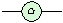
\includegraphics[width=0.5\textwidth]{chapter-1/z_rotation}
    \caption{lorum ipsum}
\end{minipage}%
\begin{minipage}{.4\textwidth}
    \centering
    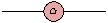
\includegraphics[width=0.46\textwidth]{chapter-1/x_rotation}
    \caption{lorum ipsum}
\end{minipage}
\end{figure}


The Pauli $Z$ and Pauli $X$ matrices are obtained by setting $\alpha = \pi$.
\begin{figure}[H]
\centering
\includezxdiagram{figures/chapter-2/pauli_z}{0.11}{
    \ket{0} \bra{0} + e^{i\pi} \ket{1} \bra{1} = 
    \begin{pmatrix} 1 & \,\,0 \\ 0 & -1 \end{pmatrix}
} \\[1ex]
\includezxdiagram{figures/chapter-2/pauli_x}{0.11}{
    \ket{+} \bra{+} + e^{i\pi} \ket{-} \bra{-} = 
    \begin{pmatrix} 0 & 1 \\ 1 & 0 \end{pmatrix}
}
\caption{Arbitrary single qubit rotations in the $Z$ and $X$ bases.}
\end{figure}

%%%

\subsubsection{Only Connectivity Matters}


\subsubsection{Composition}
We can take the matrix product by sequentially composing spiders in a ZX diagram. Note that the order of operation for matrix multiplication is from right to left, the opposite of the ZX diagram as we have defined it.

\begin{figure}[H]
    \centering
    \includezxdiagram{chapter-2/sequential}{0.27}{
        \begin{pmatrix} 1 & 0 \\ 0 & e^{i\gamma} \end{pmatrix}
        \begin{pmatrix}
            1 + e^{i\beta} & 1 - e^{i\beta} \\
            1 - e^{i\beta} & 1 + e^{i\beta}
        \end{pmatrix}
        \begin{pmatrix} 1 & 0 \\ 0 & e^{i\alpha} \end{pmatrix}}
\end{figure}

Alternatively, we could have chosen to compose the spider in parallel, resulting in the tensor product.
\begin{figure}[H]
    \centering
    \includezxdiagram{chapter-2/parallel}{0.11}{
        \begin{pmatrix} 1 & 0 \\ 0 & e^{i\alpha} \end{pmatrix} \otimes
        \begin{pmatrix}
            1 + e^{i\beta} & 1 - e^{i\beta} \\
            1 - e^{i\beta} & 1 + e^{i\beta}
        \end{pmatrix}}
\end{figure}

For instance, the CNOT gate, which is defined as the following diagram
...

Can be decomposed into matrix products and tensor products of spiders.
\begin{figure}[H]
    \centering
    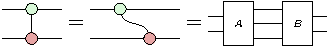
\includegraphics[width=0.65\textwidth]{chapter-2/cnot_def}
\end{figure}

\begin{figure}[H]
    \centering
    \includezxdiagram{chapter-2/A_def}{0.33}{
        \begin{pmatrix}
            1 & 0 \\
            0 & 0 \\
            0 & 0 \\
            0 & 1 \\
        \end{pmatrix} \otimes
        \begin{pmatrix} 1 & 0 \\ 0 & 1 \end{pmatrix}}
\end{figure}

\begin{figure}[H]
    \centering
    \includezxdiagram{chapter-2/B_def}{0.33}{
        \begin{pmatrix} 1 & 0 \\ 0 & 1 \end{pmatrix} \otimes \frac{1}{\sqrt 2}
        \begin{pmatrix} 1 & 0 & 0 & 1 \\ 0 & 1 & 1 & 0 \end{pmatrix}}
\end{figure}

\begin{figure}[H]
    \centering
    \includezxdiagram{chapter-2/cnot}{0.10}{
        \Bigg[
        \begin{pmatrix} 1 & 0 \\ 0 & 1 \end{pmatrix} \otimes \frac{1}{\sqrt 2}
        \begin{pmatrix} 1 & 0 & 0 & 1 \\ 0 & 1 & 1 & 0 \end{pmatrix} \Bigg]
        %
        \left[ \begin{pmatrix}
            1 & 0 \\
            0 & 0 \\
            0 & 0 \\
            0 & 1 \\
        \end{pmatrix} \otimes
        \begin{pmatrix} 1 & 0 \\ 0 & 1 \end{pmatrix} \right] =
        %
        \begin{pmatrix}
        1 & 0 & 0 & 0 \\
        0 & 1 & 0 & 0 \\
        0 & 0 & 0 & 1 \\
        0 & 0 & 1 & 0
        \end{pmatrix}}
\end{figure}

\begin{figure}[H]
    \centering
    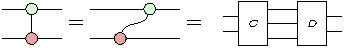
\includegraphics[width=0.65\textwidth]{chapter-2/cnot_def2}
\end{figure}

\begin{figure}[H]
\centering
\begin{minipage}{.4\textwidth}
    \centering
    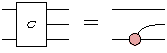
\includegraphics[width=0.80\textwidth]{chapter-2/C_def}
\end{minipage}%
\begin{minipage}{.4\textwidth}
    \centering
    \includegraphics[width=0.80\textwidth]{chapter-2/D_Def}
\end{minipage}
\end{figure}

